%%%%%%%%%%%%%%%%%%%%%%%%%%%%%%%%%%%%%%%%%
% Beamer Presentation
% LaTeX Template
% Version 1.0 (10/11/12)
%
% This template has been downloaded from:
% http://www.LaTeXTemplates.com
%
% License:
% CC BY-NC-SA 3.0 (http://creativecommons.org/licenses/by-nc-sa/3.0/)
%
%%%%%%%%%%%%%%%%%%%%%%%%%%%%%%%%%%%%%%%%%

%----------------------------------------------------------------------------------------
%	PACKAGES AND THEMES
%----------------------------------------------------------------------------------------

\documentclass{beamer}

\usepackage[utf8x]{inputenc}
\usepackage{amsmath,amsfonts,amssymb}
\usepackage{url}
\usepackage{listings}
\usepackage{moresize}
\usepackage{color}
\usepackage{moresize}
\usepackage{graphicx} % Allows including images
\usepackage{booktabs} % Allows the use of \toprule, \midrule and \bottomrule in tables
\usepackage{animate}

% Custom colors
\usepackage{color}
\definecolor{deepblue}{rgb}{0,0,0.5}
\definecolor{deepred}{rgb}{0.6,0,0}
\definecolor{deepgreen}{rgb}{0,0.5,0}

\definecolor{darkgreen}{rgb}{ 0.2968, 0.59765625, 0.0}
\definecolor{darkblue}{rgb}{ 0.0, 0.2968, 0.59765625 }
\definecolor{maroon}{rgb}{0.8,0.0,0.0}

\usetheme{Madrid}
\useinnertheme{circles}
\usecolortheme{dolphin}
\setbeamercovered{transparent}
\beamertemplatenavigationsymbolsempty

\title[SixTrackLib]{SixTrackLib: A Library for GPU Accelerated Single-Particle Tracking}
\author{Martin Schwinzerl}
\date{June 17th 2020}

\begin{document}
\begin{frame}
\begin{figure}
    \centering
    \includegraphics[width=\textwidth]{images/title.png}
\end{figure}
\end{frame}

\begin{frame}{Summary from "Introduction to GPU Programming"}
\begin{itemize}
    \item GPUs are massively parallel systems with significant single-precision and (ideally: proportionally) reduced double-precision performance
    \item Currently two main competing frameworks: OpenCL and CUDA
    \item But: highly dynamic landscape (ROCm, OneAPI, SPIR-V/PTX, ...)
    \item OpenCL and CUDA are similar $\rightarrow$ abstract away the differences
    \item $3D$ grid of threads, execute programs in lock-stop as "teams" 
    \item Segmented memory, Host $\leftrightarrow$ Device
    \item Parallel Performance:
    \begin{itemize}
        \item Sequential portion of the run-time $t_s$ is a major limiting factor
        \item Especially pertinent for GPUs: thread-deference, branching
        \item Grow problem size $N$ faster than $t_s$ $\rightarrow$ weak scaling
    \end{itemize}
\end{itemize}
\end{frame}

% ------------------------------------------------------------------------------------
% Introduction:

\begin{frame}{Introducing SixTrackLib}
\texttt{SixTrackLib} is a parallel, single particle tracking library used for simulating the trajectories of the particles forming the beam(s) in an accelerator\\[0.3cm]
\begin{itemize}
    \item Single particle: particles $P_i$ and $P_j$ with $i\neqj$ do not interact. 
    \item Tracking: via symplectic, discrete, (thin-lens) maps $\bm{M}_m$, representing the beam-element at position $m$ in the accelerator and updating the particle's state: $ P_i\left(m + 1\right) \leftarrow \bm{M}_m\left(P_i\left(m \right) \right)$
    \item Parallel: For $N_{particles} \gg 1$: "Embarrassingly" parallel problem
    \item Library: independent of application, low barrier of entry, reusable, embeddable, extensible, future backend for \texttt{SixTrack}.
\end{itemize}
\\[0.3cm]
\underline{https://github.com/SixTrack/SixTrackLib}
\end{frame}


\begin{frame}[fragile]
    \frametitle{SixTrackLib: HPC \& Design Requirements}
    \textbf{Use-Cases}: Ranging from dedicated HPC simulation tool for studies to being a potential backend for \texttt{SixTrack} in the context of the LHC@Home project\\[0.2cm]
    \begin{enumerate}
                \item {\only<1-6>{Single code-base (User API: C, C++, Python 3)}}
                      {\only<7>{\color{deepred}Single code-base (User API: C, C++, Python 3)}}
                \item<2-> Work across wide pool of hardware, different parallel back-ends 
                \item<3-> Good scalability towards high number of particles on parallel processors and GPUs
                \item<4-> High code efficiency for small(er) number of Particles using vectorised code / single thread implementation
                \item<5->{\only<5-6>{From the users perspective: single program with                   minimal changes}}
                         {\only<7>{\color{deepred}From the users perspective: single program with minimal changes}}
                \item<6->Numerical accuracy, stability \& reproducibility
        \end{enumerate}
    \\[0.3cm]
    \only<7>
    {
    Currently supported backends: OpenCL 1.2, CUDA, Single-Instruction, Multiple-Data (Auto)Vectorised Code (SIMD)
    \\[0.3cm] $\Rightarrow$ "Least Common Denominator Coding" (i.e. C99 for the shared code-base, abstractions using macros, High-Level API)
    }
\end{frame}

%\begin{frame}{Note: A Symplectic Approach To Particle Tracking}
%
%\end{frame}

%\begin{frame}{A Symplectic Approach To Particle Tracking 2}
%\end{frame}

% -----------------------------------------------------------------------------------
% Implementation and Design

\begin{frame}[label=beginintro1]
\frametitle{Implementation \& Basic Usage}
\begin{center}
    \Large{ Follow along the \texttt{introduction\_to\_sixtracklib.ipynb} for a more detailed and interactive introduction}
    \\[2em]
    \hyperlink{endintro1}{\beamerskipbutton{Skip Ahead to End of Section}}
\end{center}
\end{frame}


\begin{frame}[fragile]
\frametitle{Modelling the Particle State}
    \begin{itemize}
    \item We keep track of \textbf{21} attributes in total $\sim$ 168 Bytes / particle
    \item $6$ degrees of freedom for tracking: $x, p_x, y, p_y, \zeta, \delta$
    \item $4$ logical coordinates (\texttt{particle\_id},         
            \texttt{at\_element}, \texttt{at\_turn}, \texttt{state})
    \item $11$ attributes that are not strictly needed:
        \begin{itemize}
            \item $5$ attributes of the reference particle: 
                  $q_0, m_0, \beta_0, \gamma_0, (P_0 \cdot c)$
            \item $6$ auxiliary coordinates:
                  $s$, $p_\sigma = (E-E0)/(\beta_0 \cdot P_0 \cdot c)$, 
                  $r_{pp}=P_0/P$, $r_{vv}=\beta/\beta_0$, 
                  \texttt{charge\_ratio} $=(q/q_0)$, $\chi=(q/q_0)/(m/m_0)$
        \end{itemize}
    \item A \texttt{Particles} instance can store the state of a single particle:
    \end{itemize}
    \begin{figure}[h]
            \centering
            \includegraphics[width=\textwidth]{images/particle_state_01.png}
    \end{figure}
    \item \textbf{Note}: the state of the simulation is encapsulated in the \texttt{Particles} instance
\end{frame}

\begin{frame}{Modelling the Particle State}
\begin{itemize}
\item A \texttt{Particles} instance can also store the state of many particles:
\end{itemize}
\begin{figure}
            \centering
            \includegraphics[width=0.9\textwidth]{images/particle_state_02.png}
\end{figure}
\end{frame}

\begin{frame}{Lattice \& Beam Elements}
In General: Similar to \texttt{SixTrack} 
    \begin{itemize}
        \item \texttt{Drift}, \texttt{DriftExact}
        \item \texttt{Multipole} (incl. Dipoles, Quadrupoles, Sextupoles, etc.)
        \item \texttt{Cavity}
        \item \texttt{RFMultipole}
        \item \texttt{XYShift}: transversal shift
        \item \texttt{SRotation}: rotation in the transversal plane
        \item \texttt{BeamMonitor}: programmable dump of particle state
        \item \texttt{BeamBeam4D}, \texttt{BeamBeam6D}
        \item \texttt{SpaceChargeCoasting}, \texttt{SpaceChargeBunched}\footnote{, \texttt{SpaceChargeBunched} $\rightarrow$ \texttt{SpaceChargeQGaussian}}
        \item \texttt{DipoleEdge}
        \item \texttt{LimitRect}, \texttt{LimitEllipse}, \texttt{LimitRectEllipse}: aperature checks
        \end{itemize}
\end{frame}

\begin{frame}{Lattice \& Beam Elements}
There are different methods to get a lattice for \texttt{SixTrackLib}
\begin{enumerate}
    \item Build manually, element by element
    \item Load from binary dump 
    \item Import from \texttt{pysixtrack} \value{mysavedenumi}
    \item Import from \texttt{MAD-X} (via \texttt{pysixtrack} and \texttt{cpymad})
    \item Import from \texttt{SixTrack} (via \texttt{pysixtrack} and \texttt{sixtracktools})
\end{enumerate}
\end{frame}

\begin{frame}{SideBar: \texttt{pysixtrack}}
    \begin{itemize}
        \item \texttt{pysixtrack}: \url{https://github.com/SixTrack/pysixtrack}
        \item Minimal \& and straight forward particle tracking implementation written in Python 3 
        \item Independent of \texttt{SixTrackLib} (and \texttt{SixTrack})
        \item Idea: prototyping physics, easy to understand, duck-type-able 
        \item External Reference / Verification for \texttt{SixTrackLib}
    \end{itemize}
    \begin{figure}[h]
        \centering
        \includegraphics[width=0.95\textwidth]{images/pysixtrack_01.png}
    \end{figure}
\end{frame}

\begin{frame}{Lattice \& Beam Elements}
\begin{enumerate}
    \item Build manually, element by element
    \begin{figure}[h]
        \centering
        \includegraphics[width=0.95\textwidth]{images/lattice_01.png}
    \end{figure}
\end{enumerate}
\end{frame}

\begin{frame}{Lattice \& Beam Elements}
\begin{enumerate}
    \setcounter{enumi}{1}
    \item Load from binary dump 
    \begin{figure}[h]
        \centering
        \includegraphics[width=0.95\textwidth]{images/lattice_02.png}
    \end{figure}
\end{enumerate}

\begin{itemize}
    \item \textbf{Note}: For users of C/C++ APi, this is the recommended way to consume an imported lattice from \texttt{pysixtrack}, \texttt{MAD-X}, or \texttt{SixTrack}
    \item \textbf{Question}: What format does the binary dump have? $\Rightarrow$ Later
\end{itemize}
\end{frame}

\begin{frame}{Lattice \& Beam Elements}
\begin{enumerate}
    \setcounter{enumi}{2}
    \item Import from \texttt{pysixtrack}
    \begin{figure}[h]
        \includegraphics[width=0.95\textwidth]{images/pysixtrack_02.png}
    \end{figure}
\end{enumerate}
\begin{itemize}
    \item \texttt{pysixtrack} can use pretty much any iterable object to store a sequence of beam-elements (e.g. a \texttt{list} environment). 
    \item By using a \texttt{pysixtrack}.\texttt{Line}, we can export directly to 
          \texttt{SixTrackLib}
\end{itemize}
\end{frame}

\begin{frame}{Lattice \& Beam Elements}
\begin{enumerate}
    \setcounter{enumi}{3}
    \item Import from \texttt{MAD-X} via \texttt{pysixtrack} (and \texttt{cpymad})
    \begin{figure}[h]
        \includegraphics[width=0.85\textwidth]{images/pysixtrack_madx_01.png}
    \end{figure}
\end{enumerate}
\end{frame}

\begin{frame}{Lattice \& Beam Elements}
\begin{enumerate}
    \setcounter{enumi}{4}
    \item Import from \texttt{SixTrack} via \texttt{pysixtrack} (and \texttt{sixtracktools}\footnote{\texttt{sixtracktools} is a helper library. Cf. \url{https://github.com/SixTrack/sixtracktools}})
    \begin{figure}[h]
        \includegraphics[width=0.9\textwidth]{images/pysixtrack_sixtrack_01.png}
    \end{figure}
\end{enumerate}
\end{frame}

\begin{frame}{Example: Tracking Code Working On CPUs \& GPUs\\(With Minimal Changes)}
    \begin{figure}[h]
        \centering
        \includegraphics[width=0.95\textwidth]{images/track_example_cpu_gpu.png}
    \end{figure}
\end{frame}

\begin{frame}{Different Tracking Modes}
\begin{enumerate}
    \item \texttt{track\_until\(\)} Mode:
    \begin{figure}[h]
        \centering
        \includegraphics[width=0.9\textwidth]{images/track_modes_01.png}
    \end{figure}
    
    \item \texttt{track\_elem\_by\_elem\(\)} Mode:
    \begin{figure}[h]
        \centering
        \includegraphics[width=0.9\textwidth]{images/track_modes_02.png}
    \end{figure}
    \item \texttt{track\_line\(\)} Mode:
    \begin{figure}[h]
        \centering
        \includegraphics[width=0.9\textwidth]{images/track_modes_03.png}
    \end{figure}
\end{enumerate}
\end{frame}

\begin{frame}[label=endintro1]
    \frametitle{Implementation \& Basic Usage}
    \begin{center}
    \Large{Back from the interactive \texttt{introduction\_to\_sixtracklib.ipynb}}
    \\[2em]
    \hyperlink{beginintro1}{\beamerskipbutton{Return to Start of Previous Section}}
\end{center}
\end{frame}

\begin{frame}{Usage \& Integration Strategies For \texttt{SixTrackLib}}
Sorted in the order "easily accessible" to "complex \& invasive"
\begin{enumerate}
    \item<1->Use \texttt{track\_until\(\)}, \texttt{collect\_*}, \texttt{push_\*}
    \item<4->Use custom Kernel + Runtime Compilation + \texttt{track\_line\(\)} (Currently only OpenCL, C99)
    \item<5->Share particles state "in-place" with other applications (zero-copy) together with \texttt{track\_line\(\)} (Currently only CUDA,
    C++ or Python)
    \item<3->Implement the required functionality (e.g. "beam-elements") into \texttt{SixTrackLib} (C99 \& C++)
    \item<2->Directly link your application against the header-only subset of \texttt{SixTrackLib} (C99)
\end{enumerate}
\end{frame}

% ----------------------------------------------------------------------------------
% Performance Analysis:

\begin{frame}{Performance Analysis (CPU, Single Threaded)}
\begin{figure}[h]
    \centering 
    \includegraphics[width=1.1\textwidth]{images/performance_analysis_01.png}
\end{figure}
\end{frame}

\begin{frame}{Performance Analysis - Lin/Log Plot}
\begin{figure}[h]
    \centering 
    \includegraphics[width=1.1\textwidth]{images/performance_analysis_02.png}
\end{figure}
\end{frame}

\begin{frame}{Performance Analysis - Log/Log Plot}
\begin{figure}[h]
    \centering 
    \includegraphics[width=1.1\textwidth]{images/performance_analysis_03.png}
\end{figure}
\end{frame}

% Modes of Integration



% ----------------------------------------------------------------------------------
% Usage Examples

\begin{frame}{A Selection Of Usage Examples}
\begin{enumerate}
    \item Studying Particle Losses\newline 
          Carlo Emilio Montanari (Università di Bologna), Massimo Giovannozzi
    \item Symplectic Kicks From An Electron Cloud\newline 
          Konstantinos Paraschou (AUTH,CERN), Giovanni Iadarola, et al
    \item Simulating Beam-Beam Interactions \& Space-Charge Effects\newline 
          Hannes Bartosik, Giovanni Iadarola, et al
    \item Integrating SixTrackLib with PyHEADTAIL\newline
          Adrian Oeftiger (GSI/FAIR)
        
\end{enumerate}
\end{frame}

% Carlo Emilio:

\begin{frame}{1 Dynamic Aperture (DA), Beam-Stability, Resonances}
\begin{itemize}
    \item Study uses \texttt{SixTrackLib} directly to perform tracking for $N$ turns
    \item Performs analysis and evaluation between turns on the host 
    \item "Simple" use case - no extension and customisation was required
\end{itemize}
\begin{figure}[h]
    \includegraphics[width=0.8\textwidth]{carlo_emilio_figs/da_radial_scan.png}
    \centering 
    \caption{Sampling stable region via radial scans over $N_{turns}$}
\end{figure}

\end{frame}

\begin{frame}[fragile]
\frametitle{1 Dynamic Aperture (DA), Beam-Stability, Resonances}
\begin{itemize}
    \item Visualising $4D$ space ($\left{r, \alpha, \Theta_1, \Theta_2\right}$ is challenging - \texttt{SixTrackLib} helps with creating interactive views by being embeddable into parameterised visualisations
\end{itemize}
\only<1>
{
\begin{figure}[h]
    \includegraphics[width=0.9\textwidth]{carlo_emilio_figs/da_evolution_01.png}
    \centering 
    \caption{Evolution of $r$ over $\alpha$ for a given $\Theta_1$,$\Theta_2$ slice over $N_{turns}$}
\end{figure}
}
\only<2>
{
\begin{figure}[h]
    \includegraphics[width=0.9\textwidth]{carlo_emilio_figs/da_evolution_01_a.png}
    \centering 
    \caption{Evolution of $r$ over $\alpha$ for a given $\Theta_1$,$\Theta_2$ slice over $N_{turns}$}
\end{figure}
}
\end{frame}

\begin{frame}{1 Dynamic Aperture (DA), Beam-Stability, Resonances}
\begin{figure}
    \centering
    \includegraphics[width=0.8\textwidth]{carlo_emilio_figs/da_evolution_02.png}
    \caption{Comparison of simulated $DA(N)$ with fit $D(N) = \rho_\ast \left(\frac{\kappa}{2e}\right)^\kappa \frac{1}{\ln^\kappa\frac{N}{N_0}}$}
\end{figure}
\end{frame}

\begin{frame}[fragile]
\frametitle{1 Dynamic Aperture (DA), Beam-Stability, Resonances}
\only<1>
{
\begin{figure}
    \centering
    \includegraphics[width=0.95\textwidth]{carlo_emilio_figs/resonance_plot_01.png}
    \caption{Histogram and average measured $r$ over $\Theat_1$, $\Theta_2$ plane in dependence of initial value for $\alpha$ }
\end{figure}
}
\only<2>
{
\begin{figure}
    \centering
    \includegraphics[width=0.95\textwidth]{carlo_emilio_figs/resonance_plot_02.png}
    \caption{Histogram and average measured $r$ over $\Theat_1$, $\Theta_2$ plane in dependence of initial value for $\alpha$ }
\end{figure}
}
\only<3>
{
\begin{figure}
    \centering
    \includegraphics[width=0.95\textwidth]{carlo_emilio_figs/resonance_plot_03.png}
\end{figure}
}
\end{frame}

% Kostas: 

\begin{frame}{2 Symplectic Kicks From An Electron Cloud}
\begin{columns}
\column{0.5\textwidth}
For various reasons and under certain conditions (fulfilled in the LHC), there exists a complex distribution of electrons within the vacuum chamber that interacts with the beam called \textbf{``{\color{blue}Electron Cloud}''}.
%Positively charged, bunched beams can create, trap and multiply electrons in the beam chamber, giving rise to what is called ``{\color{blue}Electron Cloud}'' --- a complex distribution of electrons that interacts with the beam.  

Distribution {\color{red}strongly depends on x, y and time!} (as bunch passes through the electron cloud)
\column{0.5\textwidth}

\begin{figure}
    \footnotesize
    Example PyECLOUD simulation:
    \centering
    \includegraphics[width=\textwidth]{kostas_figs/rho_pinch_beam_sigma.png}
\end{figure}
\vspace{-0.4cm}
    \hfill \tiny Particles with an amplitude of 1 beam-$\sigma$  \\ \hfill  oscillate within the black line
    
\normalsize
 
\end{columns}
\vspace{0.1cm}
Under usual approximations\textsuperscript{0} the interaction can be written as a {\color{blue}thin-lens through the Hamiltonian}: 
\vspace{-0.7cm}
\begin{equation*}\hspace{3cm}
    H(x,y,\tau;s) = 
    \frac{qL}{\beta_0 P_0 c}
    \phi \left(x,y,\tau\right) \delta (s)
\end{equation*}
\vspace{-0.5cm}

where $\phi$ is the scalar potential describing the electron cloud.

\footnotetext[0]{see \href{https://cds.cern.ch/record/2684858}{G. Iadarola, CERN-ACC-NOTE-2019-0033.}}
\end{frame}

\begin{frame}{2 Symplectic Kicks From An Electron Cloud}
\begin{itemize}
    \item PyECLOUD would produce $\phi$ on a discrete grid (x, y, time)\\
    $\rightarrow$ $\phi$ should be \textbf{interpolated}
    \item To study slow effects, interpolation should produce symplectic kicks \\
    %simplest scheme 
    $\rightarrow$  Tricubic Interpolation: $\phi(x,y,\tau) = \sum_{i,j,k=0}^3 a_{ijk} x^i y^j \tau^k$
    \item Add custom beam-element \texttt{TriCub} to implement the map
    \item $N^3$ coefficients with typically $N\sim \mathcal{O}(10^2)$ per \texttt{TriCub} element 
          $\Rightarrow \mathcal{O}(10^3)$ MByte of data for each \texttt{TriCub}
    \item But: interpolation data can be shared between many beam-elements (e.g. All focusing quadrupole magnets have similar Electron Cloud)
    \item \textbf{Idea:} implement infrastructure to store data externally from \texttt{TriCub} elements and assign \& share coefficient data
\end{itemize}
\begin{center}
\includegraphics[width=0.7\textwidth]{kostas_figs/tricub_tricubdata_overview.png}
\end{center}
\end{frame}

%\begin{frame}{2 Symplectic Kicks From An Electron Cloud}
%\includegraphics[width=\textwidth]{kostas_figs/tricub_impl_05.png}
%\end{frame}

\begin{frame}{2 Symplectic Kicks From An Electron Cloud}
\begin{itemize}
    \item In principle, TriCub element general enough to describe any interaction whose Hamiltonian can be discretized on a grid of (x,y,$\tau$) 
    %(e.g. 6D beam-beam and space charge effects with arbitrary profiles)
    \item GPUs: large global memory (4-16 GByte), adequate memory bandwidth
    $\rightarrow$ perfect environment for simulations with TriCub beam-elements.
\end{itemize}

\end{frame}

% Hannes / Gianni:

\begin{frame}{3 Beam-Beam Interactions \& Space-Charge Effects}
\begin{itemize}
    \item  \texttt{SixTrackLib} implements $4D$ and $6D$ beam-beam (BB) interactions using a weak-strong beam formulation\footnote{G. Iadarola et al. CERN-ACC-NOTE-2018-0023 "6D beam-beam interaction step-by-step}
    \item Frozen Space-Charge (SC) beam-elements share infrastructure with the BB implementation
    \begin{itemize}
        \item Coasting \texttt{SpaceChargeCoasting}
        \item Bunched \texttt{SpaceChargeQGaussianProfile}
        \item Bunched \texttt{SpaceChargeInterpolatedProfile} using linear and cubic spline longitudinal interpolation (under development)
    \end{itemize}        
    \item \texttt{SpaceChargeInterpolatedProfile} uses API to assign external data to a number of beam-elements to share profile samples and interpolation parameters between SC elements
\end{itemize}
\end{frame}

\begin{frame}{3 Beam-Beam Interactions \& Space-Charge Effects}
\begin{itemize}
    \item A closer look on the performance data $\Longrightarrow$
    \item BB and SC implementations impact run-time performance even if no elements are present in the lattice!
\end{itemize}
\begin{figure}[h]
    \centering
    \includegraphics[width=\textwidth]{images/performance_analysis_04.png}
\end{figure}
\end{frame}

\begin{frame}{3 Beam-Beam Interactions \& Space-Charge Effects}
\begin{itemize}
    \item Calculation of field components (according to a Gaussian distribution) and the complex error function (Faddeeva function) is shared between BB and SC elements
\end{itemize}
\includegraphics[width=0.8\textwidth]{beam_fields_figs/fadeeva_03.png}
\end{frame}

\begin{frame}[fragile]
\only<1>{
 \begin{figure}
     \centering
     \includegraphics[width=0.85\textwidth]{beam_fields_figs/20191105_SC_and_ripple_02.png}
 \end{figure}
}
\only<2>{
\begin{figure}
     \centering
\includegraphics[width=0.85\textwidth]{beam_fields_figs/20191105_SC_and_ripple_03.png}
\end{figure}
}
\footnotetext[2]{
H. Bartosik, F. Schmidt "Studies on Tune Ripple", \newline4th ICFA Mini-Workshop on SpaceCharge 2019, \url{https://indico.cern.ch/event/828559/contributions/3528378}}
\end{frame}



%Adrian:

\begin{frame}{4 Integrating \texttt{SixTrackLib} with \texttt{PyHEADTAIL}}
    Beyond the single-particle treatment within \texttt{SixTrackLib}, model collective effects as ``true'' interaction between macro-particles via \texttt{PyHEADTAIL}\footnote[frame]{\url{https://github.com/PyCOMPLETE/PyHEADTAIL}}:
    \begin{itemize}
        \item accelerated on the GPU via (Py)CUDA
        \item self-consistent models for  (e.g.\ 3D PIC/particle-in-cell) space charge, wake fields and feedback systems
    \end{itemize}
    
    \begin{columns}
        \begin{column}[b]{0.45\linewidth}
            \begin{figure}
                \includegraphics[width=\linewidth]{adrian_figs/Adrian_Fig3-624x435.png}
                \caption{PIC space charge}
            \end{figure}
        \end{column}
        \hfill
        \begin{column}[b]{0.45\linewidth}
            \begin{figure}
                \includegraphics[width=\linewidth]{adrian_figs/wakefield.pdf}
                \caption{wake fields}
            \end{figure}
        \end{column}
    \end{columns}
\end{frame}

\begin{frame}{4 Integrating \texttt{SixTrackLib} with \texttt{PyHEADTAIL}}

    Share particle memory between  \texttt{SixTrackLib} and  \texttt{PyHEADTAIL}:
    \begin{enumerate}
        \item use  \texttt{SixTrackLib}'s \texttt{track\_line} API to advance particles through parts of accelerator lattice
        \item expose particle coordinates on GPU via SixTrackLib's \texttt{get\_particle\_addresses} interface to apply kick in PyHEADTAIL
        \item[$\Longrightarrow$] alternating single- and multi-particle physics while \emph{remaining} on GPU device memory!
    \end{enumerate}
    
    \begin{figure}
        \centering
        \includegraphics[width=0.5\linewidth]{adrian_figs/transverse-model.pdf}
        % \caption{alternating}
    \end{figure}
\end{frame}

{
\setbeamercolor{block body}{bg=white}
\setbeamercolor{alertblock body}{bg=white}
\setbeamercovered{invisible}
\begin{frame}{Applications of  \texttt{SixTrackLib} +  \texttt{PyHEADTAIL}}
    \begin{columns}
        \begin{column}[T]{0.48\linewidth}
            \begin{block}{\centering 90 deg stop-band}
                Interplay of coherent vs.\ incoherent resonances driven by space charge
                \begin{figure}
                    \centering
                    \includegraphics[width=\linewidth]{adrian_figs/k0xy93p5_k0z1to3_particlemotion_interm.png}
                    \caption{running 3D PIC in FODO}
                \end{figure}
            \end{block}
        \end{column} \hfill
        \begin{column}[T]{0.48\linewidth}
            \begin{block}{\centering FAIR synchrotron SIS100}
                Beam loss studies with space charge and nonlinear magnet imperfections
                \begin{figure}
                    \centering
                    \includegraphics[width=\linewidth]{adrian_figs/tunescan_detailed.png}
                    \caption{frozen SC in SIS100 lattice}
                    \label{fig:my_label}
                \end{figure}
            \end{block}
        \end{column}
    \end{columns}
    
    \pause
    \vspace{-5cm}
    
    \begin{columns}\hspace*{0.02\linewidth}
        \begin{column}[T]{0.44\linewidth}
            \begin{alertblock}{\centering run time}
                \centering
                % 8 million macro-particles, \break 10'000 cells: $<4$h \break on NVIDIA RTX 2080 Ti (consumer-grade GPU)
                1 million macro-particles, \break 5'000 cells: $<20$min on \break NVIDIA V100 (high-end GPU)
            \end{alertblock}
        \end{column}
        \hspace*{0.02\linewidth}
        \hfill
        \hspace*{0.02\linewidth}
        \begin{column}[T]{0.44\linewidth}
            \begin{alertblock}{\centering run time}
                \centering
                1000 macro-particles, \break 20'000 turns: $<3$min on \break NVIDIA V100 (high-end GPU)
            \end{alertblock}
        \end{column}
        \hspace*{0.02\linewidth}
    \end{columns}
            
    \vspace{5cm}
\end{frame}
}

\begin{frame}{Thank You For Your Attention!}
\begin{itemize}
    
    \item \texttt{SixTrackLib} available from \url{https://github.com/SixTrack/sixtracklib}\\[1em]
    
    \item Presentation, Jupyter-Notebooks, Images, Data available via 
    \url{https://github.com/martinschwinzerl/sixtracklib-presentations/tree/master/20200617_hss_section_meeting_sixtracklib}\\[1em]
          
    \item \textbf{Info:} Friday, June 19th, 2020, 14:30 s.t.: BE Seminar Talk about \texttt{SixTrackLib} $\longrightarrow$ \url{https://indico.cern.ch/event/929467/}\\[1em]
    
\end{itemize}
\end{frame}

\end{document}

